\documentclass{beamer}
\mode<presentation>
\usepackage{amsmath}
\usepackage{amssymb}
%\usepackage{advdate}
\usepackage{adjustbox}
\usepackage{subcaption}
\usepackage{enumitem}
\usepackage{multicol}
\usepackage{gensymb}
\usepackage{mathtools}
\usepackage{listings}
\usepackage{url}
\def\UrlBreaks{\do\/\do-}
\usetheme{Boadilla}
\usecolortheme{lily}
\setbeamertemplate{footline}
{
  \leavevmode%
  \hbox{%
  \begin{beamercolorbox}[wd=\paperwidth,ht=2ex,dp=1ex,right]{author in head/foot}%
    \insertframenumber{} / \inserttotalframenumber\hspace*{2ex} 
  \end{beamercolorbox}}%
  \vskip0pt%
}
\setbeamertemplate{navigation symbols}{}

\providecommand{\nCr}[2]{\,^{#1}C_{#2}} % nCr
\providecommand{\nPr}[2]{\,^{#1}P_{#2}} % nPr
\providecommand{\mbf}{\mathbf}
\providecommand{\pr}[1]{\ensuremath{\Pr\left(#1\right)}}
\providecommand{\qfunc}[1]{\ensuremath{Q\left(#1\right)}}
\providecommand{\sbrak}[1]{\ensuremath{{}\left[#1\right]}}
\providecommand{\lsbrak}[1]{\ensuremath{{}\left[#1\right.}}
\providecommand{\rsbrak}[1]{\ensuremath{{}\left.#1\right]}}
\providecommand{\brak}[1]{\ensuremath{\left(#1\right)}}
\providecommand{\lbrak}[1]{\ensuremath{\left(#1\right.}}
\providecommand{\rbrak}[1]{\ensuremath{\left.#1\right)}}
\providecommand{\cbrak}[1]{\ensuremath{\left\{#1\right\}}}
\providecommand{\lcbrak}[1]{\ensuremath{\left\{#1\right.}}
\providecommand{\rcbrak}[1]{\ensuremath{\left.#1\right\}}}
\theoremstyle{remark}
\newtheorem{rem}{Remark}
\newcommand{\sgn}{\mathop{\mathrm{sgn}}}
\providecommand{\abs}[1]{\left\vert#1\right\vert}
\providecommand{\res}[1]{\Res\displaylimits_{#1}} 
\providecommand{\norm}[1]{\lVert#1\rVert}
\providecommand{\mtx}[1]{\mathbf{#1}}
\providecommand{\mean}[1]{E\left[ #1 \right]}
\providecommand{\fourier}{\overset{\mathcal{F}}{ \rightleftharpoons}}
%\providecommand{\hilbert}{\overset{\mathcal{H}}{ \rightleftharpoons}}
\providecommand{\system}{\overset{\mathcal{H}}{ \longleftrightarrow}}
	%\newcommand{\solution}[2]{\textbf{Solution:}{#1}}
%\newcommand{\solution}{\noindent \textbf{Solution: }}
\providecommand{\dec}[2]{\ensuremath{\overset{#1}{\underset{#2}{\gtrless}}}}
\newcommand{\myvec}[1]{\ensuremath{\begin{pmatrix}#1\end{pmatrix}}}
\let\vec\mathbf

\lstset{
%language=C,
frame=single, 
breaklines=true,
columns=fullflexible
}

\numberwithin{equation}{section}

\title{12.9.7.15 Presentation}
\author{G. Abhimanyu Koushik \\ EE24BTECH11024}

\date{\today} 
\begin{document}

\begin{frame}
\titlepage
\end{frame}

\section*{Outline}
\begin{frame}
\tableofcontents
\end{frame}
\section{Problem}
\begin{frame}
\frametitle{Problem Statement}
%
The population of a village increases continuously at the rate proportional to the number of its inhabitants present at any time. If the population of the village was 20,000 in 1999 and 25,000 in the year 2004, what will be the population of the village in 2009?
%
\end{frame}

%\subsection{Literature}
\section{Solution}
\subsection{Input Parameters}
\begin{frame}
\frametitle{Input Parameters}
%\framesubtitle{Literature}
\begin{table}[H]    
  \centering
  \begin{tabular}[12pt]{ |c| c|}
    \hline
    \textbf{Variable} & \textbf{Description}\\
    \hline
    $n$ & Order of given differential equation\\
    \hline
    $a_i$ & Coeefficient of $i$th derivative of the function in the equation\\
    \hline
    $c$ & constant in the equation\\
    \hline
    $y^i$ & $i$th derivative of given function\\
    \hline
    $\vec{y}\brak{t}$ & $\myvec{c \\ y\brak{t} \\ y^\prime\brak{t} \\ \vdots \\ y^{n-1}\brak{t}}$\\
    \hline
    $h$ & stepsize, taken to be 0.001\\
    \hline
    $u\brak{x}$ & Unit step function\\
    \hline
    \end{tabular}

\end{table}
\end{frame}
\subsection{Laplace Transform properties}
\begin{frame}
\frametitle{Laplace Transform properties}
%\framesubtitle{Literature}
Properties of Laplace tranform
\begin{align}
	\mathcal{L}\brak{y^{\prime}} &= s\mathcal{L}\brak{y} -y\brak{0}\\
	\mathcal{L}\brak{1} &= \frac{1}{s}\\
	\mathcal{L}\brak{cf\brak{t}} &= c\mathcal{L}\brak{f\brak{t}}\\
	\mathcal{L}\brak{f\brak{t}} = F\brak{s} &\implies \mathcal{L}\brak{e^{at}f\brak{t}} = F\brak{s-a}	
\end{align}
\end{frame}
\subsection{Equation solving}
\begin{frame}
\frametitle{Equation solving}
Applying the properties to the given equation
\begin{align}
	y^{\prime} &= k_{0}y\\
	\mathcal{L}\brak{y^\prime} - \mathcal{L}\brak{k_{0}y}&= 0\\
	s\mathcal{L}\brak{y} - y\brak{0} - k_{0}\mathcal{L}\brak{y} &= 0\\
	\mathcal{L}\brak{y} &= \frac{y\brak{0}}{s - k_{0}}\\
	y &= y\brak{0}e^{k_{0}x}u\brak{x}
\end{align}
Taking 1999 to be the initial year, we get $y\brak{0} = 20000$ and $y\brak{5} = 25000$\\
\end{frame}
\begin{frame}
Substituting the initial conditions gives
\begin{align}
	y\brak{0} &= 20000\\
	y\brak{5} &= 25000\\
	20000e^{5k_{0}} &= 25000\\
	e^{5k_{0}} &= \frac{5}{4}\\
	5k_{0} &= \ln{\frac{5}{4}}\\
	k_{0} &= \frac{1}{5}\ln{\frac{5}{4}}
\end{align}
The theoritical solution is 
\begin{align}
	f\brak{x} &= 20000e^{\frac{1}{5}\brak{\ln{\frac{5}{4}}}x}u\brak{x}\\
	f\brak{x} &= 20000\brak{\frac{5}{4}}^{\frac{x}{5}}u\brak{x	}
\end{align}
Substituting $x=10$ gives 31250
\end{frame}


\subsection{Computational Solution}
\begin{frame}
\frametitle{Computational Solution}
First we have to find the $k$ value in the differential equation, for that
\begin{align}
	y\brak{t+h} &= y\brak{t} + hy^\prime\brak{t}\\
	y\brak{t+h} &= y\brak{t} + hk_{0}y\brak{t}\\
	y\brak{t+2h} &= y\brak{t+h} + hk_{0}y\brak{t+h}\\
	y\brak{t+2h} &= y\brak{t} + hk_{0}y\brak{t} + hk_{0}\brak{y\brak{t} + hk_{0}y\brak{t}}\\
	y\brak{t+2h} &= \brak{1+hk_{0}}^2y\brak{t}
\end{align}
Similarly
\begin{align}
	y\brak{t+nh} &= \brak{1+hk_{0}}^ny\brak{t}
\end{align}
\end{frame}
\begin{frame}
Subtituting the initial condition and value of $h$ gives
\begin{align}
	y\brak{5} &= \brak{1+0.001k_{0}}^{5000}y\brak{0}\\
	25000 &= 20000\brak{1+0.001k_{0}}^{5000}\\
	\brak{\frac{5}{4}}^{\frac{1}{5000}} - 1 &= 0.001k_{0}\\
	k_{0} &= \frac{\brak{\frac{5}{4}}^{\frac{1}{5000}} - 1}{0.001}\\
	k_{0} &\approx 0.04462
\end{align}
\end{frame}
\begin{frame}
Consider the given linear differential equation
\begin{align}
	a_{n}y^n + a_{n-1}y^{n-1} + \dots + a_{1}y^\prime + a_{0}y + c = 0
\end{align}
Then
\begin{align}
	y^{\prime}\brak{t} = \lim_{h\to 0}\frac{y\brak{t+h} - y\brak{t}}{h}\\
	y\brak{t+h} = y\brak{t} + hy^{\prime}\brak{t}
\end{align}
Similarly
\begin{align}
	y^{i}\brak{t+h} &= y^{i}\brak{t} + hy^{i+1}\brak{t}\\
	y^{n-1}\brak{t+h} &= y^{n-1}\brak{t} + hy^{n}\brak{t}\\
	y^{n-1}\brak{t+h} &= y^{n-1}\brak{t} + h\brak{-\frac{a_{n-1}}{a_n}y^{n-1}-\frac{a_{n-2}}{a_n}y^{n-2} - \dots -\frac{a_{0}}{a_n}y - \frac{c}{a_n}}
\end{align}
\end{frame}
\begin{frame}
Where i ranges from 0 to $n-1$\\
\begin{align}
	\vec{y}\brak{t+h} = \vec{y}\brak{t} + \myvec{0 & 0 & 0 & 0 & \dots & 0 & 0\\ 0 & 0 & 1 & 0 & \dots & 0 & 0\\0 & 0 & 0 & 1 & \dots & 0 & 0\\\vdots & \vdots & \vdots & \vdots& \ddots & \vdots & \vdots\\
	0 & 0 & 0 & 0 & \dots & 0 & 1\\-\frac{1}{a_n} & -\frac{a_0}{a_n} & -\frac{a_1}{a_n} & -\frac{a_2}{a_n} & \dots & -\frac{a_{n-2}}{a_n} & -\frac{a_{n-1}}{a_n}}\brak{h\vec{y}\brak{t}}\\
	\vec{y}\brak{t+h} = \myvec{1 & 0 & 0 & 0 & \dots & 0 & 0\\ 0 & 1 & h & 0 & \dots & 0 & 0\\0 & 0 & 1 & h & \dots & 0 & 0\\\vdots & \vdots & \vdots & \vdots& \ddots & \vdots & \vdots\\
	0 & 0 & 0 & 0 & \dots & 1 & h\\-\frac{h}{a_n} & -\frac{a_0h}{a_n} & -\frac{a_1h}{a_n} & -\frac{a_2h}{a_n} & \dots & -\frac{a_{n-2}h}{a_n} & 1-\frac{a_{n-1}h}{a_n}}\brak{\vec{y}\brak{t}}
\end{align}
\end{frame}
\begin{frame}
Discretizing the steps gives us
\begin{align}
	\vec{y}_{k+1} = \myvec{1 & 0 & 0 & 0 & \dots & 0 & 0\\ 0 & 1 & h & 0 & \dots & 0 & 0\\0 & 0 & 1 & h & \dots & 0 & 0\\\vdots & \vdots & \vdots & \vdots& \ddots & \vdots & \vdots\\
	0 & 0 & 0 & 0 & \dots & 1 & h\\-\frac{h}{a_n} & -\frac{a_0h}{a_n} & -\frac{a_1h}{a_n} & -\frac{a_2h}{a_n} & \dots & -\frac{a_{n-2}h}{a_n} & 1-\frac{a_{n-1}h}{a_n}}\brak{\vec{y}_{k}}
\end{align}
where $k$ ranges from 0 to number of data points with $y^{i}_0$ being the given initial condition and vector $\vec{y}_0 = \myvec{c\\y\brak{0}\\y^\prime\brak{0}\\\vdots\\y^{n-1}\brak{0}}$
\end{frame}
\begin{frame}
For the given question\\
\begin{align}
	\vec{y}_{k+1} = \myvec{1 & 0\\ -h & 1+hk_0}\vec{y}_k
\end{align}
Record the $y_k$ for 
\begin{align}
x_k =lowerbound+kh
\end{align}
and then plot the graph. The result will be as given below.\\
The codes below verifies the obtained solution. 
\end{frame}
%\section{Plot}
\section{Plot of the function}
\begin{frame}
\frametitle{Plot of the function}
\begin{figure}[H]
    \centering
	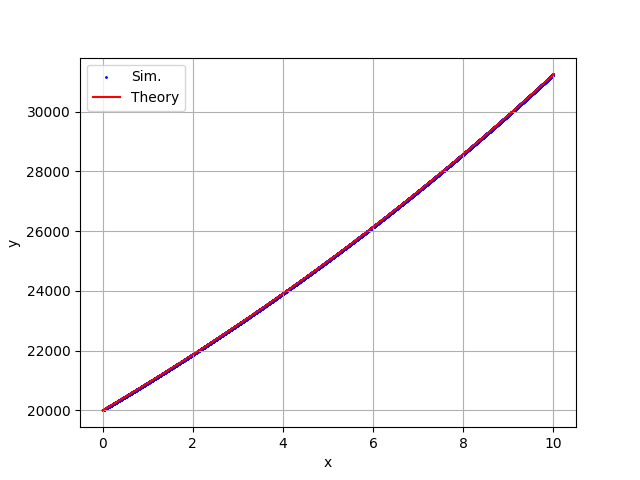
\includegraphics[width=0.8\columnwidth]{figs/fig.png}
    \caption{Function satisfying given differential equation}
    \end{figure}   
\end{frame}
\section{C Code}
\begin{frame}[fragile]
\frametitle{C Code}
\begin{lstlisting}[language=C]
#include <stdio.h>
#include <stdlib.h>
#include <math.h>
#include "functions.h"
double** matrixgen(int order, double coefficients[order+2], double stepsize){
	double** outputmatrix = identity(order+1);
	for(int i=1; i<order; i++){
		outputmatrix[i][i+1] = stepsize;
	}
	outputmatrix[order][0] = -1/coefficients[0]*stepsize;
	for(int i=1; i<order+1; i++){
		outputmatrix[order][i] = (-coefficients[order+1-i]/coefficients[0])*stepsize;
	}
	outputmatrix[order][order] += 1; 
	return outputmatrix;}

\end{lstlisting}
\end{frame}
\begin{frame}[fragile]
\begin{lstlisting}[language=C]

double* recorddata(double lowerbound, double upperbound, int order,  double coefficients[order+2], double initialconditions[order], double stepsize){
	double** vector_y = createMat(order+1,1);
	vector_y[0][0] = coefficients[order+1];
	for(int i=0;i<order;i++){
		vector_y[i+1][0] = initialconditions[i];
	}
	double** matrix = matrixgen(order, coefficients, stepsize);
	int no_datapoints = ((upperbound-lowerbound)/stepsize);
	double* yvalues = malloc(no_datapoints*sizeof(double));
	for(int i = 0; i<no_datapoints; i++){
		vector_y = Matmul(matrix,vector_y,order+1,order+1,1);
		yvalues[i] = vector_y[1][0];
	}
	return yvalues;
}


\end{lstlisting}
\end{frame}

\section{Python Code}
\begin{frame}[fragile]
\frametitle{Python Code for Plotting}
\begin{lstlisting}[language=Python]
import ctypes
import numpy as np
import matplotlib.pyplot as plt

# Load the shared library
solver = ctypes.CDLL('./solver.so')

# Define the function signatures
solver.recorddata.restype = ctypes.POINTER(ctypes.c_double)
solver.recorddata.argtypes = [
    ctypes.c_double,  # lowerbound
    ctypes.c_double,  # upperbound
    ctypes.c_int,     # order
    ctypes.POINTER(ctypes.c_double),  # coefficients
    ctypes.POINTER(ctypes.c_double),  # initialconditions
    ctypes.c_double   # stepsize
]

\end{lstlisting}
\end{frame}
\begin{frame}[fragile]
\begin{lstlisting}[language=Python]

# Define parameters
order =1
lowerbound = 0.0
upperbound = 10.0
stepsize = 0.001
y_0 = 20000
k = (((5/4)**(1/5000)) - 1)/0.001
coefficients = np.array([1.0, -k, 0.0], dtype=np.double) 
initialconditions = np.array([y_0, k*y_0], dtype=np.double)

# Calculate the number of data points
no_datapoints = int((upperbound - lowerbound) / stepsize)

# Call the C function
results_ptr = solver.recorddata(
    ctypes.c_double(lowerbound),
    ctypes.c_double(upperbound),
    ctypes.c_int(order),
    coefficients.ctypes.data_as(ctypes.POINTER(ctypes.c_double)),
    initialconditions.ctypes.data_as(ctypes.POINTER(ctypes.c_double)),

\end{lstlisting}
\end{frame}
\begin{frame}[fragile]
\begin{lstlisting}[language=Python]
    ctypes.c_double(stepsize)
)
# Convert results back to a NumPy array
results = np.ctypeslib.as_array(results_ptr, shape=(no_datapoints,))
# Generate x-values for plotting
x_values = np.arange(lowerbound + stepsize, upperbound + stepsize, stepsize)
y_function = 20000*((5/4)**(x_values/5))
# Plot the data
plt.scatter(x_values, results, color='blue', s=1, label='Sim.')
plt.plot(x_values, y_function, color='red', label='Theory')
plt.xlabel('x')
plt.ylabel('y')
plt.legend()
plt.grid(True)
plt.savefig('../figs/fig.png')
plt.show()
\end{lstlisting}
\end{frame}
\end{document}

